\subsection{Product Perspective}
\subsubsection{Scenarios}
\textbf{Student edits his profile} \newline
A student decides to enhance their chances of finding an internship by creating a detailed profile. They access using their academic credentials and start the profile editing. They upload a CV to make it available to companies and list their skills, which will be used by the platform to find the best matching internship. After submitting the changes, the system analyzes it and suggests improvements, such as adding missing skills or refining the description of experiences. At any time the student can update his profile. \\\\
\textbf{Student searches and applies for an internship} \newline
A student is eager to find an internship aligned with their career aspirations. He explores the available opportunities by filtering results based on their interests and skill requirements. The results of these operations are ordered based on the match between the requested skills and the ones specified in his profile. Once they find a suitable internship, they review the project details carefully and submit their application. The system forwards their CV to the company for evaluation.\\\\
\textbf{The system recommends internships to a student}\\
After completing their profile and specifying their skills and preferences, such as desired fields or specific technologies, a student receives notifications from the system whenever an internship aligns with their profile. The student reviews these recommendations and selects the most relevant opportunities to apply for.\\\\
\textbf{Company posts an internship project}\\
A company wants to post an internship project on the platform in order to attract qualified candidates. To do this it logs in and from its dashboard selects the section “Create a new internship”. From this section the company sets the following info about the project: 
\begin{itemize}
    \item A (unique) title to identify the project.
    \item A description to explain in more detail what the internship is about.
    \item The terms of the internship, such as the retribution or the work hours.
    \item A set of tags that specify which skills are better suited for the offer.
\end{itemize}
Once  this step is completed, the user can see the posting from a dedicated section in the dashboard.\\\\
\textbf{The System Recommends Candidates to Companies}\\
After companies post internship opportunities, the system analyzes the profiles of students who have expressed interest in internships. Based on the skills, qualifications, and preferences of both the students and the internships, the system sends notifications to companies when candidates who match their requirements are available. Companies can then review the recommended student profiles and decide whether to proceed with the selection process. Once a company selects a candidate from the recommended list, the system notifies the student and updates the status of the internship accordingly. The company can then initiate the selection process, which may involve interviews or assessments, to finalize the decision.\\\\
\textbf{A company receives an application and starts an interview}\\
Once a student applies for an internship, the company is notified and begins the selection process. To assess if the candidate is a good fit, the company reviews the candidate’s profile, including the CV. For a better evaluation of aspects that may not be covered by the first step, the company can create questionnaires through a dedicated section in its profile. The candidate has then to answer to them through the platform. These interviews may involve structured questionnaires or discussions aimed at gauging the candidate’s skills, motivation, and suitability for the role. The system supports the company by helping schedule interviews, managing the process, and collecting answers from the student. It also stores feedback and assessment results to assist the company in making an informed decision. After the interviews, the company determines whether to proceed with the candidate and updates the status of the internship accordingly. The student is then notified about the outcome and provided with next steps for finalizing the internship agreement.\\\\
\textbf{A company accepts a candidate for an internship}\\
After evaluating applications and conducting interviews or assessments, a company identifies the most suitable candidate for an internship position. The company confirms their choice by notifying the candidate through the platform. The system updates the status of the internship to reflect the selection, and the student receives a confirmation along with any necessary next steps to finalize the agreement.\\\\
\textbf{Improving Student Profiles and CVs}\\
The system reviews student profiles and identifies opportunities for improvement. It suggests refining CV descriptions, highlighting key achievements, or adding new skills to align better with the needs of prospective internship postings. These recommendations help students present themselves as stronger candidates.\\\\
\textbf{A student posts feedback about an internship}\\
A student has ended an internship and since he had a very positive experience, he decides to leave some feedback to let others know about it. He can add a rating from 1 to 5 stars and, optionally, leave a textual comment where he can explain in more detail the reasons for his rating.\\\\
\textbf{Optimizing Internship Descriptions}\\
The system evaluates internship postings to ensure they are clear and appealing to potential applicants. It might recommend refining project details, adjusting skill requirements to better match available candidates, or emphasizing benefits such as mentorship opportunities or financial compensation. These enhancements increase the visibility and attractiveness of the internship.\\\\
\textbf{A company leaves feedback about an internship}\\
After the completion of an internship, a company that has worked with a student decides to leave feedback  to let others know about the performance. The company can add a rating from 1 to 5 stars and, optionally, leave a textual comment where he can explain in more detail the reasons for his rating.\\\\
\textbf{Handling a complaint during an internship}\\
During an internship, issues may arise, such as unclear project requirements, insufficient support from the company, or performance concerns from either the student or the company. Both parties, students and companies, can report problems through the platform. The system ensures that complaints are properly recorded and escalated to the relevant university representatives for resolution. If necessary, the internship is paused or terminated, and both the student and the company are notified. The university then coordinates the resolution process, ensuring that any serious concerns are addressed promptly.\\\\
\textbf{Monitoring an ongoing internship}\\
During an internship, issues may arise, such as unclear project requirements, insufficient support from the company, or performance concerns from either the student or the company. Both parties, students and companies, can report problems through the platform. The system ensures that complaints are properly recorded and escalated to the relevant university representatives for resolution. If necessary, the internship is paused or terminated, and both the student and the company are notified. The university then coordinates the resolution process, ensuring that any serious concerns are addressed promptly.\\\\
\subsubsection{Domain Class Diagram}
\begin{figure}[h]
    \centering
    
\includegraphics[width=\linewidth]{Images/diagram.drawio.png}
    \caption{Domain class diagram}
    \label{fig:enter-label}
\end{figure}
The figure above presents the domain class diagram.  Company, Student, and University represent distinct user types, each a subclass of an abstract User class.  A company offers internships to which multiple students may apply.  Each interview is associated with a single student and internship, encompassing multiple questions. Following an interview, a contract, referencing a single internship and student, is generated; its status is tracked via the associated InternshipStatus.\\\\
To register a complaint, report an issue, or submit information, users must initiate a discussion thread to facilitate communication among relevant stakeholders.  Upon resolution, the initiating user will close the thread and mark it as resolved.\\\\
Should a consensus remain elusive, the university may terminate the internship by modifying the student's enrollment status.\\\\
The Affinity Analyzer quantifies the compatibility between a student and an internship, considering the student's CV, internship specifications, and prior feedback from both student and company regarding other internships.\\\\
The CVAnalyzer offers recommendations for CV enhancement based on a comparative analysis of other CVs and internships.\\\\
The InternshipAnalyzer provides feedback on optimizing internship descriptions by referencing other internships and student CVs.
\subsubsection{State Diagrams}
\begin{figure}[h]
    \centering
    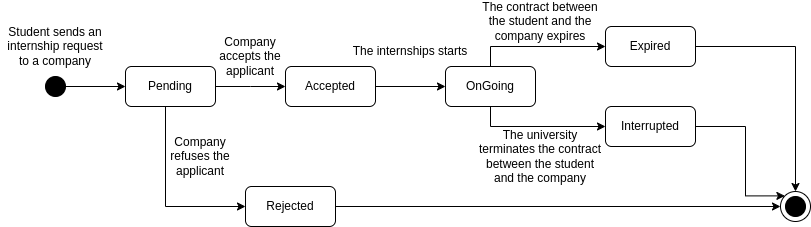
\includegraphics[width=\textwidth]{Images/state_diagram.png}
    \caption{Contract lifecycle state diagram}
    \label{fig:state-diagram}
\end{figure}
One of the most important aspect of Students\&Companies is the internships' management. In \ref{fig:state-diagram} are illustrated the steps followed by the contracts. Note that \textit{Pending} means that the student has applied for an internship and if the company accepts their application, possibly after a round on interviews, the internship can start.
\subsection{Product Functions}
In this section the functions provided by the system are described to be categorized by user.
\subsubsection{Student}
    \paragraph{Login\\}
    The system allows students to log on to the platform using their academic credentials.
    \paragraph{Edit Profile\\}
    The system allows students to edit their profile.
    \paragraph{Internship recommendation\\}
    This function allows students to receive an email notification when an internship that could interest them becomes available.
    \paragraph{Search an internships\\}
    This function enables students to search for internships using keyword filters.
    \paragraph{Apply for an internship\\}
    This function allows the student to apply for an internship.
    \paragraph{Answer interview questions\\}
    This function enables students contacted by the company to answer structured questionnaires.
    \paragraph{Consulting CV suggestions\\}
    Students can view system-generated suggestions on how to improve their CVs to make them more attractive to companies.
\subsubsection{Company}
    \paragraph{Registration and login}
    The application allows companies to register and become users.  Registration requires the company to provide its name and tax identification number (P. IVA number), [altre informazioni?].  This information is mandatory; incomplete submissions will result in registration failure.
    \paragraph{Upload an internship\\}
    This function allows logged-in companies to create new internship posts. They do this by inserting mandatory data, including the internship type, duration, and whether it is paid, along with optional information.
    \paragraph{Student recommendation\\}
    This function allows companies to receive an email notification when a student CVs corresponding to their needs becomes available.
    \paragraph{Interview students\\}
    This function allows companies to interview students by proposing structured questionnaires.
    \paragraph{Create contract\\}
    This function allows companies to register the start of an internship by saving the contract signed by both parties and other optional information.
\subsubsection{University}
    \paragraph{Login\\}
    The system allows universities to log into the platform using the credentials given by S\&C at the stipulation of the partnership.
    \paragraph{Terminate an internship\\}
    This function allows university supervisors to terminate an internship by changing its status to "terminated" when an agreement cannot be reached.
\subsubsection{Students and Companies}
    \paragraph{Give feedback about an internship\\}
    This feature allows both students and companies to post feedback about internships, which includes a required rating and an optional textual comment.
    \paragraph{Open discussion\\}
    Users may initiate discussions with interested parties.
\subsubsection{Everyone}
    \paragraph{Send and receive messages within a discussion\\}
    This function allows the user involved in a discussion to exchange messages with other interested parties.
    \paragraph{Monitor the status of the internship\\}
    This function allows the user to see the status of an internship in which he’s involved.
\subsection{User Characteristic}
There are three types of users that interact with the Platform: student, company and university.
\subsubsection{Student}
University students seeking internships. They can actively search for internships or receive automated recommendations.
\subsubsection{Company}
Company is a user who can create an internship and interview students with structured questionnaires. This type of user can also start a discussion.
\subsubsection{University}
University is a user who can interact with students and companies in a discussion and end an internship when needed.
\subsection{Assumptions, Dependencies and Constraints}
\subsubsection{Regulatory Policies}
S\&C complies with GDPR, CCPA, and other applicable data protection laws.
Personal data (students, companies, universities) is collected and processed transparently, only for purposes such as managing internships.
\subsubsection{Domain Assumptions}
\begin{domain-assumptions}
    \item Students create their CVs.
    \item Companies properly insert information about internships.
    \item Universities interfere with the contract between students and companies when needed.
    \item Notifications must arrive to the target users.
    \item Students have an academic credential.
    \item University is available on the SheerID API.
    \item Students are enrolled in a university registered on SheerID.
    \item Users who register as a company have a valid VAT number.
    \item Users who register as a company have a valid VAT number.
\end{domain-assumptions}